\documentclass[12pt]{article}
\usepackage{graphicx}
\usepackage{amsmath}

\usepackage[margin=1in]{geometry}
\usepackage{float}
\usepackage{listings}
\usepackage{booktabs}

\title{Labwork 8: Scatter}
\author{Ngo Quang Truong 2540106}
\date{3 Oct 2026}

\begin{document}

\maketitle
\newpage

\section{Introduction}
This report presents two scatter kernels on GPU: \texttt{RGB2HSV()} converts an RGB image to HSV, and \texttt{HSV2RGB()} converts it back.

\section{Method}
The RGB image is stored as an \textbf{Array of Structs (AoS)}: one array \texttt{img[y, x, c]} where the 3 channels of a pixel sit next to each other. The HSV result is stored as a \textbf{Struct of Arrays (SoA)}: three separate 2D arrays \texttt{H[y, x]}, \texttt{S[y, x]}, \texttt{V[y, x]}.

Both kernels use a $16\times16$ thread block, one thread per pixel. Test image: a $3840\times2160$ RGB image.

\section{RGB to HSV}
Each thread reads its pixel, scales $R, G, B$ to $[0, 1]$, and computes $max$, $min$ and $\Delta = max - min$:
\begin{equation}
H = \begin{cases}
0^\circ & \Delta = 0 \\
60^\circ \times (\frac{G-B}{\Delta} \bmod 6) & max = R \\
60^\circ \times (\frac{B-R}{\Delta} + 2) & max = G \\
60^\circ \times (\frac{R-G}{\Delta} + 4) & max = B
\end{cases}
\quad
S = \begin{cases} 0 & max = 0 \\ \frac{\Delta}{max} & max \neq 0 \end{cases}
\quad
V = max
\end{equation}
The ``mod 6'' is done by adding $360^\circ$ when $H$ is negative. The thread then \textbf{scatters} the three values into the three output arrays:
\begin{lstlisting}[language=Python, basicstyle=\ttfamily\small]
H[y, x] = h
S[y, x] = s
V[y, x] = mx
\end{lstlisting}

\section{HSV to RGB}
Each thread reads $H, S, V$ from the three arrays and computes
\begin{equation}
d = H/60,\quad hi = \lfloor d \rfloor \bmod 6,\quad f = d - \lfloor d \rfloor
\end{equation}
\begin{equation}
l = V(1-S),\quad m = V(1-fS),\quad n = V(1-(1-f)S)
\end{equation}
$(R, G, B)$ is picked from $(V,n,l)$, $(m,V,l)$, $(l,V,n)$, $(l,m,V)$, $(n,l,V)$, $(V,l,m)$ depending on $hi$. It is scaled back to $[0, 255]$ (rounded) and written into the single RGB array.

\section{Results}
The image was converted to HSV and back to RGB, and the output was compared with the input. The maximum per-channel difference is \textbf{0}, so the round trip is exact.

\begin{figure}[H]
    \centering
    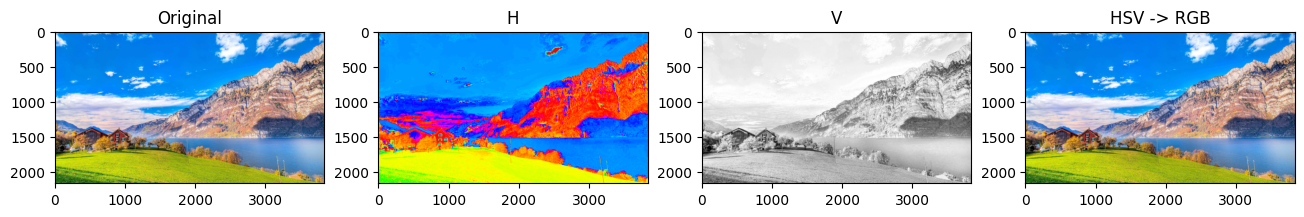
\includegraphics[width=\textwidth]{hsv_output.png}
    \caption{Original, H channel, V channel, and image converted back to RGB}
    \label{fig:hsv}
\end{figure}

\end{document}
